\documentclass[aspectratio=169,10pt]{beamer}

% ------------------------------------------------------------------
% Packages & TikZ Library
% ------------------------------------------------------------------
\usepackage{tikz}
\usepackage{booktabs}
\usepackage{amsmath,amssymb}
\usepackage{xcolor}
\usepackage{array,colortbl}
\usepackage{multirow}
\usepackage{microtype}

\usetikzlibrary{arrows.meta, positioning, shapes.geometric, fit, calc, backgrounds, decorations.pathreplacing, matrix}

% ------------------------------------------------------------------
% Colour palette
% ------------------------------------------------------------------
\definecolor{cbBlue}   {RGB}{31,119,180}
\definecolor{cbOrange} {RGB}{214,95,14}
\definecolor{cbGreen}  {RGB}{44,160,44}
\definecolor{cbRed}    {RGB}{200,40,40}
\definecolor{cbPurple} {RGB}{130,80,170}
\definecolor{cbBrown}  {RGB}{130,76,60}
\definecolor{lBlue}    {RGB}{215,232,250}
\definecolor{lOrange}  {RGB}{255,228,195}
\definecolor{lGreen}   {RGB}{208,242,210}
\definecolor{lPurple}  {RGB}{234,218,252}
\definecolor{lRed}     {RGB}{252,215,215}
\definecolor{lGray}    {RGB}{242,242,242}
\definecolor{dkGray}   {RGB}{70,70,70}

% ------------------------------------------------------------------
% Beamer theme settings
% ------------------------------------------------------------------
\usetheme{default}
\setbeamercolor{frametitle}{bg=cbBlue,fg=white}
\setbeamerfont{frametitle}{size=\large,series=\bfseries}
\setbeamertemplate{navigation symbols}{}
\setbeamertemplate{footline}{\hfill{\color{dkGray}\tiny\insertframenumber/\inserttotalframenumber\hspace{4pt}}\vspace{3pt}}

\newcommand{\sectionbox}[2]{\tikz{\node[fill=#1,rounded corners=2pt,text=white,font=\tiny\bfseries,inner sep=3pt]{#2};}}

\title[PowerSim]{\textbf{PowerSim}: Simulation-Based Power Framework}
\subtitle{Architecture, Configuration \& Simulation Pipeline}
\author{PowerSim Framework}
\date{2026}

\begin{document}

% TITLE SLIDE
\begin{frame}[plain]
  \centering
  \vspace{1.2cm}
  {\color{cbBlue}\Huge\bfseries PowerSim}\\[4pt]
  {\large Simulation-Based Power Assessment for\\ Differential Circadian Rhythm Analysis}\\[16pt]
  
\begin{tikzpicture}\draw[cbBlue, line width=2pt] (0,0) -- (10,0);\end{tikzpicture}\\[12pt]
  {\footnotesize\color{dkGray}George's Overview $\cdot$ 2026}
\end{frame}

% SLIDE 1: PIPELINE
\begin{frame}{Step 1 | Detailed Simulation Pipeline}
\centering
\tikzset{
    input/.style={rectangle, rounded corners=2pt, draw=cbBlue, fill=lBlue, text width=2.8cm, font=\scriptsize\bfseries, align=center, minimum height=0.6cm},
    engine/.style={rectangle, draw=dkGray, fill=lGray, text width=2.6cm, font=\scriptsize, align=center, minimum height=0.6cm},
    proc/.style={rectangle, rounded corners=5pt, draw=cbOrange, fill=lOrange, text width=2.8cm, font=\scriptsize\bfseries, align=center, minimum height=0.7cm},
    output/.style={rectangle, draw=cbGreen, fill=lGreen, text width=2.2cm, font=\scriptsize\bfseries, align=center},
    ARR/.style={-{Stealth[scale=0.8]}, thick, dkGray}
}
\begin{tikzpicture}[node distance=0.5cm and 1.0cm]
  \node[input] (bio) {CircadianBioOptions};
  \node[input, below=of bio] (des) {CircadianDesignOptions};
  \node[input, below=of des] (ana) {CircadianAnalysisOptions};
  \node[proc, right=1.2cm of des] (rpa) {runPowerAnalysis()};
  \node[engine, right=0.8cm of rpa, yshift=0.5cm] (sim) {simCircadianDiff()};
  \node[engine, below=0.3cm of sim] (det) {Method Detection};
  \begin{scope}[on background layer]
    \node[draw=dkGray, dashed, fill=white, fit=(sim) (det), inner sep=10pt, label={[font=\tiny, dkGray]north:Iterate $N$ Sims}] (loopbox) {};
  \end{scope}
  \node[proc, right=0.8cm of loopbox] (strat) {stratified\_power()};
  \node[output, above right= -0.2cm and 0.8cm of strat] (curves) {Power Curves};
  \node[output, below= 0.2cm of curves] (fdr) {FDR Tables};
  \draw[ARR] (bio.east) -- (rpa.west); \draw[ARR] (des.east) -- (rpa.west); \draw[ARR] (ana.east) -- (rpa.west);
  \draw[ARR] (rpa.east) -- (loopbox.west); \draw[ARR] (sim.south) -- (det.north); \draw[ARR] (loopbox.east) -- (strat.west);
\end{tikzpicture}
\end{frame}

% SLIDE 2: CONFIGURATION OBJECTS (UPDATED WITH ALL PARAMETERS)
\begin{frame}{Step 2 | Configuration Objects \& Detailed Parameters}
\begin{columns}[T,onlytextwidth]
% BIO OPTIONS
\begin{column}{0.38\textwidth}
  \begin{block}{CircadianBioOptions()}
    \tiny
    \begin{tabular}{lp{3.5cm}}
        \toprule
        \textbf{Parameter} & \textbf{Role} \\
        \midrule
        \texttt{amplitude} & Dist. (scalar/vector/fn/pilot) \\
        \texttt{phase} & Phase dist. (or "uniform") \\
        \texttt{lBaselineExpr} & Log baseline expression dist. \\
        \texttt{lOD} & Over-dispersion (noise) dist. \\
        \texttt{phase\_diff} & DP shift range (e.g. \texttt{c(-6, 6)}) \\
        \texttt{amp\_diff} & DA fold-change (e.g. \texttt{c(0.5, 2)}) \\
        \texttt{dr\_amp\_scale} & Scale on Amp for DR effect size \\
        \texttt{dr\_sigma\_scale} & Scale on Noise for DR effect size \\
        \texttt{dp\_shift\_mode} & "fixed" vs "uniform" assignment \\
        \texttt{sim.seed} & Reproducibility (N-dependent) \\
        \bottomrule
    \end{tabular}
  \end{block}
\end{column}

% DESIGN OPTIONS
\begin{column}{0.28\textwidth}
  \begin{block}{DesignOptions()}
    \tiny
    \begin{tabular}{lp{2cm}}
        \toprule
        \textbf{Parameter} & \textbf{Role} \\
        \midrule
        \texttt{cts} & Pilot TOD (if passive) \\
        \texttt{test\_types} & \texttt{c("DR","DP","DA")} \\
        \texttt{sample\_sizes} & Sweep range \\
        \texttt{nsims} & Iteration count \\
        \bottomrule
    \end{tabular}
  \end{block}
  \vspace{0.2cm}
  \textit{\tiny Note: Active designs default to evenly spaced collection times.}
\end{column}

% ANALYSIS OPTIONS
\begin{column}{0.32\textwidth}
  \begin{block}{AnalysisOptions()}
    \tiny
    \begin{tabular}{lp{2.5cm}}
        \toprule
        \textbf{Parameter} & \textbf{Role} \\
        \midrule
        \texttt{p.adjust.method} & Correction (default "BH") \\
        \texttt{parallel.ncores} & Parallel threads \\
        \texttt{target\_effect} & Min effect size threshold \\
        \texttt{fdr\_thresholds} & Reported alpha levels \\
        \texttt{reference\_n} & Visualisation anchor size \\
        \texttt{phase\_shifts} & Sensitivity sweep mags \\
        \texttt{amp.cutoff} & DCP pre-filter min amp \\
        \bottomrule
    \end{tabular}
  \end{block}
\end{column}
\end{columns}
\end{frame}

% SLIDE 3: MATHEMATICAL ENGINE
\begin{frame}{Step 3 | The Generative Model}
\begin{columns}[T]
    \column{0.5\textwidth}
    \sectionbox{cbBlue}{Cosinor Simulation Equation}
    \small
    $$y_{g,i,k} = M_g + A_{g,k} \cos\left(\frac{2\pi}{24}t_i - \phi_{g,k}\right) + \epsilon_{g,i,k}$$
    
    \scriptsize
    \textbf{Learned from Pilot Data:}
    \begin{itemize}
        \item $M_g$: MESOR (Baseline expression)
        \item $A_{g,k}$: Amplitude (Circadian strength)
        \item $\phi_{g,k}$: Acrophase (Peak time)
    \end{itemize}
    \column{0.5\textwidth}
    \sectionbox{cbOrange}{The SNR Metric ($r$)}
    \small
    $$r = \text{Amplitude} / \text{Noise} (\sigma)$$
    \begin{block}{Why Stratify by $r$?}
        \scriptsize
        Power is non-uniform across the transcriptome. PowerSim bins results by SNR:
        \begin{itemize}
            \item \textbf{Low SNR}: $r < 1.0$
            \item \textbf{High SNR}: $r > 2.0$
        \end{itemize}
    \end{block}
\end{columns}
\end{frame}

% SLIDE 4: GENE TYPE LOGIC
\begin{frame}{Step 4 | Gene Type Assignment Logic}
\centering
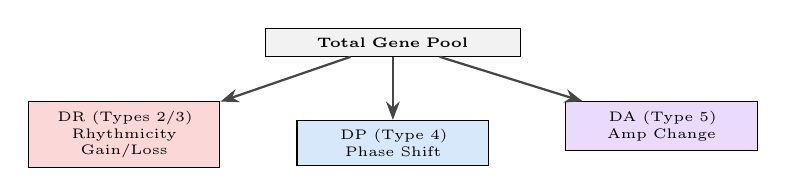
\begin{tikzpicture}[node distance=0.8cm, font=\tiny, ARR/.style={-{Stealth},thick,dkGray}]
    \node[draw, fill=lGray, text width=3cm, align=center] (pool) {\textbf{Total Gene Pool}};
    \node[draw, fill=lRed, below left=0.8cm of pool, text width=2.2cm, align=center] (dr) {DR (Types 2/3)\\Rhythmicity Gain/Loss};
    \node[draw, fill=lBlue, below=0.8cm of pool, text width=2.2cm, align=center] (dp) {DP (Type 4)\\Phase Shift};
    \node[draw, fill=lPurple, below right=0.8cm of pool, text width=2.2cm, align=center] (da) {DA (Type 5)\\Amp Change};
    \draw[ARR] (pool) -- (dr); \draw[ARR] (pool) -- (dp); \draw[ARR] (pool) -- (da);
\end{tikzpicture}
\vspace{0.3cm}
\begin{table}
    \tiny
    \begin{tabular}{lllc}
        \toprule
        \textbf{Type} & \textbf{Group 1} & \textbf{Group 2} & \textbf{Significance} \\
        \midrule
        Type 0 & Arrhythmic & Arrhythmic & Baseline Null \\
        \rowcolor{lRed!50} Type 2/3 & Rhythmic & Arrhythmic & \textbf{DR} \\
        \rowcolor{lBlue!50} Type 4 & Rhythmic & Rhythmic (Shifted) & \textbf{DP} \\
        \rowcolor{lPurple!50} Type 5 & Rhythmic & Rhythmic (Scaled) & \textbf{DA} \\
        \bottomrule
    \end{tabular}
\end{table}
\end{frame}

% SLIDE 5: DETECTION LOGIC
\begin{frame}{Step 5 | Detection Logic: DR, DP, and DA}
\centering
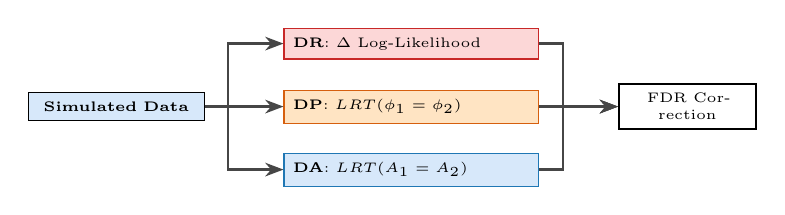
\begin{tikzpicture}[node distance=0.4cm and 0.7cm, font=\tiny, ARR/.style={-{Stealth},thick,dkGray}]
    \node[draw, fill=lBlue, text width=2cm, align=center] (data) {\textbf{Simulated Data}};
    \node[draw=cbRed, fill=lRed, right=1cm of data, yshift=0.8cm, text width=3cm] (dr) {\textbf{DR}: $\Delta$ Log-Likelihood};
    \node[draw=cbOrange, fill=lOrange, right=1cm of data, text width=3cm] (dp) {\textbf{DP}: $LRT(\phi_1 = \phi_2)$};
    \node[draw=cbBlue, fill=lBlue, right=1cm of data, yshift=-0.8cm, text width=3cm] (da) {\textbf{DA}: $LRT(A_1 = A_2)$};
    \node[draw, thick, right=1cm of dp, text width=1.5cm, align=center] (bh) {FDR Correction};
    \draw[ARR] (data.east) -- ++(0.3,0) |- (dr.west); \draw[ARR] (data.east) -- (dp.west); \draw[ARR] (data.east) -- ++(0.3,0) |- (da.west);
    \draw[ARR] (dr.east) -- ++(0.3,0) |- (bh.west); \draw[ARR] (dp.east) -- (bh.west); \draw[ARR] (da.east) -- ++(0.3,0) |- (bh.west);
\end{tikzpicture}
\begin{block}{Validation Criteria}
    \scriptsize A discovery is a \textbf{True Positive} if adjusted $p < \alpha$ and the gene matches the Ground Truth assignment from Step 4.
\end{block}
\end{frame}

% SLIDE 6: OUTPUTS
\begin{frame}{Final Output | Stratified Power Analysis}
\begin{columns}[T]
    \column{0.5\textwidth}
    \textbf{Marginal vs. Stratified Power}
    \begin{itemize}
        \scriptsize
        \item \textbf{Marginal}: Often inflated by high-amplitude genes.
        \item \textbf{Stratified}: Provides a realistic view of power per SNR bin ($r$).
    \end{itemize}
    
    \column{0.5\textwidth}
    \textbf{Data Structure}
    \tiny
    \begin{table}
        \begin{tabular}{lp{3.5cm}}
            \toprule
            \textbf{Component} & \textbf{Description} \\
            \midrule
            \texttt{power\_summary} & Power and FDR per $(N, r)$. \\
            \texttt{sensitivity} & Power vs Phase Shift magnitude. \\
            \texttt{settings} & Object snapshot for reproducibility. \\
            \bottomrule
        \end{tabular}
    \end{table}
\end{columns}
\end{frame}

% SLIDE 7: ACTIVE VS PASSIVE
\begin{frame}{Study Design | Active vs. Passive Sampling}
\begin{columns}[T]
    \column{0.45\textwidth}
    \begin{block}{Active Design (Balanced)}
        \scriptsize Spaced evenly (e.g., every 4h). Optimal for circadian parameter estimation.
    \end{block}
    \begin{block}{Passive Design (Clinical)}
        \scriptsize Based on pilot TOD (clinic hours). Often results in \textbf{Temporal Gaps}.
    \end{block}
    \column{0.55\textwidth}
    \centering \textbf{The TOD Gap Problem}
    
    \scriptsize \textcolor{cbRed}{\textbf{Impact:}} PowerSim quantifies the "Sample Size Penalty" required for clinical cohorts.
\end{columns}
\end{frame}

% SLIDE 8: SENSITIVITY
\begin{frame}{Sensitivity Sweep | Phase Shift Magnitude}
\begin{columns}[c]
    \column{0.5\textwidth}
    \scriptsize
    \textbf{Detectability Limits}: How small of a shift can we find?\\
    \begin{itemize}
        \item \texttt{phase\_shifts}: Mags swept in analysis.
        \item \texttt{target\_effect}: Minimum biological significance.
    \end{itemize}
    \column{0.5\textwidth}
    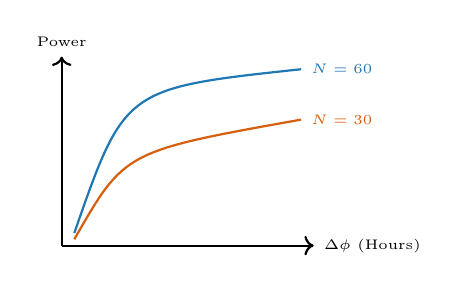
\begin{tikzpicture}[scale=0.8]
        \draw[thick, ->] (0,0) -- (4,0) node[right] {\tiny $\Delta \phi$ (Hours)};
        \draw[thick, ->] (0,0) -- (0,3) node[above] {\tiny Power};
        \draw[cbBlue, thick] (0.2,0.2) .. controls (1,2.5) .. (3.8,2.8) node[right] {\tiny $N=60$};
        \draw[cbOrange, thick] (0.2,0.1) .. controls (1,1.5) .. (3.8,2.0) node[right] {\tiny $N=30$};
    \end{tikzpicture}
\end{columns}
\end{frame}

% SLIDE 9: BENCHMARK
\begin{frame}{Benchmarking | DCP vs. CircaCompare}
\centering
\scriptsize
\begin{tabular}{lll}
    \toprule
    \textbf{Feature} & \textbf{DCP (LRT)} & \textbf{CircaCompare (NLS)} \\
    \midrule
    \textbf{Computation} & High Speed ($<10$s) & Moderate ($\sim 2$min) \\
    \textbf{Robustness} & Sensitive to balance & Robust to uneven TOD \\
    \textbf{Application} & Large-scale sweeps & Specific $N$ validation \\
    \bottomrule
\end{tabular}
\end{frame}

\end{document}